\documentclass[
  bibliography=totoc,     % Literatur im Inhaltsverzeichnis
  captions=tableheading,  % Tabellenüberschriften
  titlepage=firstiscover, % Titelseite ist Deckblatt
]{scrartcl}

% Paket float verbessern
\usepackage{scrhack}

% Warnung, falls nochmal kompiliert werden muss
\usepackage[aux]{rerunfilecheck}

% deutsche Spracheinstellungen
\usepackage{polyglossia}
\setmainlanguage{german}

% unverzichtbare Mathe-Befehle
\usepackage{amsmath}
% viele Mathe-Symbole
\usepackage{amssymb}
% Erweiterungen für amsmath
\usepackage{mathtools}

% Fonteinstellungen
\usepackage{fontspec}
% Latin Modern Fonts werden automatisch geladen

\usepackage[
  math-style=ISO,    % ┐
  bold-style=ISO,    % │
  sans-style=italic, % │ ISO-Standard folgen
  nabla=upright,     % │
  partial=upright,   % ┘
  warnings-off={           % ┐
    mathtools-colon,       % │ unnötige Warnungen ausschalten
    mathtools-overbracket, % │
  },                       % ┘
]{unicode-math}

% traditionelle Fonts für Mathematik
\setmathfont{Latin Modern Math}
\setmathfont{XITS Math}[range={scr, bfscr}]
\setmathfont{XITS Math}[range={cal, bfcal}, StylisticSet=1]

% Zahlen und Einheiten
\usepackage[
  locale=DE,                 % deutsche Einstellungen
  separate-uncertainty=true, % immer Fehler mit \pm
  per-mode=reciprocal,       % ^-1 für inverse Einheiten
]{siunitx}

% chemische Formeln
\usepackage[
  version=4,
  math-greek=default, % ┐ mit unicode-math zusammenarbeiten
  text-greek=default, % ┘
]{mhchem}

% richtige Anführungszeichen
\usepackage[autostyle]{csquotes}

% schöne Brüche im Text
\usepackage{xfrac}

% Standardplatzierung für Floats einstellen
\usepackage{float}
\floatplacement{figure}{htbp}
\floatplacement{table}{htbp}

% Floats innerhalb einer Section halten
\usepackage[
  section, % Floats innerhalb der Section halten
  below,   % unterhalb der Section aber auf der selben Seite ist ok
]{placeins}

% Seite drehen für breite Tabellen
\usepackage{pdflscape}

% Captions schöner machen.
\usepackage[
  labelfont=bf,        % Tabelle x: Abbildung y: ist jetzt fett
  font=small,          % Schrift etwas kleiner als Dokument
  width=0.9\textwidth, % maximale Breite einer Caption schmaler
]{caption}
% subfigure, subtable, subref
\usepackage{subcaption}

% Grafiken können eingebunden werden
\usepackage{graphicx}
% größere Variation von Dateinamen möglich
\usepackage{grffile}

% schöne Tabellen
\usepackage{booktabs}

% Verbesserungen am Schriftbild
\usepackage{microtype}

% Literaturverzeichnis
\usepackage[
  backend=biber,
]{biblatex}
% Quellendatenbank
\addbibresource{lit.bib}
\addbibresource{programme.bib}

% Hyperlinks im Dokument
\usepackage[
  unicode,        % Unicode in PDF-Attributen erlauben
  pdfusetitle,    % Titel, Autoren und Datum als PDF-Attribute
  pdfcreator={},  % ┐ PDF-Attribute säubern
  pdfproducer={}, % ┘
]{hyperref}
% erweiterte Bookmarks im PDF
\usepackage{bookmark}

% Trennung von Wörtern mit Strichen
\usepackage[shortcuts]{extdash}

\author{
  Ksenia Klassen
  \texorpdfstring{
    \\
    \href{mailto:ksenia.klassen@udo.edu}{ksenia.klassen@udo.edu}
  }{}%
  \texorpdfstring{\and}{, }
  Dag-Björn Hering%
  \texorpdfstring{
    \\
    \href{mailto:dag.hering@udo.edu}{dag.hering@udo.edu}
  }{}%
}
\publishers{TU Dortmund – Fakultät Physik}

\setlength{\parindent}{0pt}%keine einrückung nach absätzen

\usepackage{longtable}% bessere tabellen


\subject{V25}
\title{Der Stern-Gerlach Versuch}
\date{
  Durchführung: 24.07.2017
  \hspace{3em}
  Abgabe: 26.08.2017
}

\begin{document}

\maketitle
\thispagestyle{empty}
\tableofcontents
\newpage

\section{Theorie}
\label{sec:Theorie}
\subsection{Magnetische Momente und Drehimpulse}
Ein Hüllenelektron besitzt zwei Drehimpulse, den Spin $\vec{s}$ und den Bahndrehimpuls $\vec{l}$.
Deren Beträge sind wie folgt definiert durch die Quantenzahlen $\textit{l}$ und $s$:
\begin{align}
  |\vec{l}|&=\sqrt{\textit{l}(\textit{l}+1)\hbar}\,\,\,\,\,\text{mit $\textit{l}=0,1,...n-1$ }\\
  |\vec{s}|&=\sqrt{s(s+1)\hbar}\,\,\,\,\,\text{mit $s=\frac{1}{2}$}\
\end{align}
Den beiden Drehimpulsen kann ein magnetischen Moment zugeordnet werden:
\begin{align}
  \vec{\mu_\mathrm{\textit{l}}}&=-\mu_\mathrm{B}\sqrt{\textit{l}(\textit{l}+1)}\vec{\textit{l}_\mathrm{e}}\\
  \vec{\mu_\mathrm{s}}&=-\mu_\mathrm{B} g_\mathrm{s}\sqrt{s(s+1)}\vec{s_\mathrm{e}}
\end{align}
Es besteht eine Proportionalität zum Bohrschen-Magneton $\mu_\mathrm{B}:=\frac{1}{2}e_\mathrm{0}\frac{\hbar}{m_\mathrm{0}}$
(mit $e_\mathrm{0}$ der Elektronenladung und $m_\mathrm{0}$ der Elektronenmasse).
Die magnetische Anomalie des Elektons sorgt für den zusätzlichen Faktor $g_\mathrm{s}=2$
im magnetischen Moment des Spins.

\subsection{Wechselwirkung der Drehimpulse}
Die Wechselwirkung von Bahndrehimpulsen und Spins kann auf komplizierte Weise ablaufen.
In der Natur treten zwei Grenzfälle auf, die im Folgenden thematisiert werden:\\
\\
\textbf{1.Fall:} Bei leichten Atomen setzen sich die einzelnen Bahndrehimpulse und Spins
zu einem Gesamtbahndrehimpuls der Elektronenhülle $\vec{L}=\sum_i l_i$
bzw. Gesamtspin der Elektronenhülle $\vec{S}=\sum_i s_i$ zusammen.
Der Gesamtdrehimpuls hat den Betrag
\begin{align}
 |\vec{L}|=\sqrt{L(L+1)\hbar}
\end{align}
und ist eine quantisierte Größe:
$L$ ist ganzzahlig und nimmt die Werte $0,1,2 ,\ \text{oder} ,\ 3$ an.
Ähnlich sieht es bei dem Gesamtspin aus, der Betrag entspricht
\begin{align}
 |\vec{S}|=\sqrt{S(S+1)\hbar}
\end{align}
mit der Quantenzahl $S$. Die kann Werte von $\frac{N}{2} ,\ \text{bis} ,\ 0$
($N$ ist die Anzahl der Elektronen in den nicht abgeschlossenen Schalen)
in halbzahligen Schritten annehmen.
Diese beiden Größen koppeln zu einem Gesamtdrehimpuls der Elektronenhülle $\vec{J}$ über die sogenannte LS-Kopplung:
\begin{align}
  \vec{J}=\vec{L}+\vec{S} ,\,\,\,\,\, \text{mit dem Betrag}\,\,\,\,\,|\vec{J}|=\sqrt{J(J+1)\hbar}.
\end{align}\\
\textbf{2.Fall:} Bei schweren Atomen ist die Wechselwirkung zwischen dem Spin und
Bahndrehimpuls eines einzelnen Elektrons größer als zwischen allen Elektronen.
Es entsteht kein Gesamtbahndrehimpuls bzw. Gesamtspin.
Bahndrehimpulse $\vec{\textit{l}_\mathrm{i}}$ und Spins $\vec{s}_\mathrm{i}$ der einzelnen Elektronen ergeben
die Gesamtdrehimpulse $\vec{j}_\mathrm{i}=\vec{\textit{l}_\mathrm{i}}+\vec{s}_\mathrm{i}$ der Elektronen.
Erst die Summe aller $\vec{j}_\mathrm{i}$ ergibt den Gesamtdrehimpuls der Elektronenhülle:
\begin{align}
\vec{J}=\sum_i \vec{j}_i.
\end{align}\\
Für mittelschwere Atome besteht ein fließender Übergang.
\\
Das gesamte magnetische Moment $\vec{\mu}$ zum Gesamtdrehimpuls $\vec{J}$ ergibt sich aus der Vektorsumme der magnetischen Momente
\begin{align}
 \vec{\mu_\mathrm{L}}&=\mu_\mathrm{B}\sqrt{L(L+1)}\
 \intertext{und}\
 \vec{\mu_\mathrm{S}}&=\mu_\mathrm{B}g_\mathrm{s}\sqrt{S(S+1)}.
\end{align}
Die Richtungen von $\vec{\mu}$ und $\vec{J}$ fallen nicht zusammen, jedoch kann
gezeigt werden, dass der zu $\vec{J}$ parallele Anteil von $\vec{\mu}$ beiträgt.
Diese und weitere Überlegungen führen zum Betrag des magnetischen Momentes:
\begin{align}
  |\vec{\mu}_\mathrm{J}|\approx \mu_\mathrm{B}\sqrt{J(J+1)}\underbrace{\frac{3J(J+1)+S(S+1)-L(L+1)}{2J(J+1)}}_{g_\mathrm{J}}\label{eqn:lande}
\end{align}
Hierbei bezeichnet $g_\mathrm{J}$ den Landé-Faktor.
Unter deim Einfluss eines B-Feldes nehmen die Winkel zwischen $\vec{\mu}$ und $\vec{B}$ Werte an,
bei denen die Komponente $\mu_\mathrm{J_\mathrm{z}}$ in Feldrichtung ein ganzzahliges Vielfaches
von $g_\mathrm{J}\mu_\mathrm{B}$ ergibt.
Diese sogenannte Richtungsquantelung kann ausgedrückt werden durch:
\begin{align}
  \mu_\mathrm{J_\mathrm{z}}= -mg_\mathrm{J}\mu_\mathrm{B},
\end{align}
die ganzzahlige größe $m$ beschreibt die Orientierungsquantenzahl und hat einen Wertevorrat von
$-J$ bis $J$.
Es existieren $2J+1$ Einstellungen des magnetischen Momentes relativ zur äußeren Feldrichtung und
damit eine Aufspltung eines Nivaus in $2J+1$ Unterniveaus.
\subsection{Auswahlregeln}
Zwischen den Zuständen sind Übergänge unter der Emission eines Photons möglich.
Die Energie des Photos, damit auch die Wellenlänge der messbaren Spektrallinie,
entspricht dabei der Energiedifferenz der beiden Zustände.
%%%%%%%%%%%%%%%%%%%%%%%%%%%%%%%Rechnung
Aus Rechnungen folgen Auswahlregeln für die Übergänge.
Übergänge zwischen den Zuständen sind danach nur möglich wenn die
Orientierungsquantenzahl $m$ sich um $\pm 1$ oder gar nicht ändert:
\begin{align}
  \Delta m = 0,\pm 1.
\end{align}
\subsection{Normaler Zeemann-Effekt}
Beim normalen Zeemann-Effekt entspricht $S=0$ für alle $J:g_\mathrm{j}=1$,
dies bedeutet die Unabhängigkeit der Verschiebung der Energieniveaus von den Quantenzahlen.
Für jedes $L$ und $S$ gilt:
\begin{align}
  \Delta E=m\mu_\mathrm{B}B ,\,\,\,\,\ \text{für}\,\-J < m < J. \label{eqn:landean}
\end{align}
Es findet die Aufspaltung in die äquidistanten Unterniveaus statt, dies geschiecht auch im Angeregten Zustand.
Ein Übergang nach den Auswahlregeln kann somit stattfinden.
Die Aufspaltung und möglichen Übergänge sind in Abbildung \ref{fig:normal} dargestellt.
Die Übergänge lassen sich anhand ihrer Polarisation kategorisieren:
\begin{itemize}
  \item{$\sigma^+$-Übergang: $\Delta m_\mathrm{J}=+1$  entspricht rechtszirkularer Polarisation um das Magnetfeld}
  \item{$\sigma^-$-Übergang: $\Delta m_\mathrm{J}=-1$) entspricht linkszirkularer Polarisation um das Magnetfeld }
  \item{$\pi$-Übergang: $\Delta m_\mathrm{J}=0$ entspricht linearer Polarisation in Magnetfeldrichtung}
\end{itemize}
\begin{figure}
   \centering
    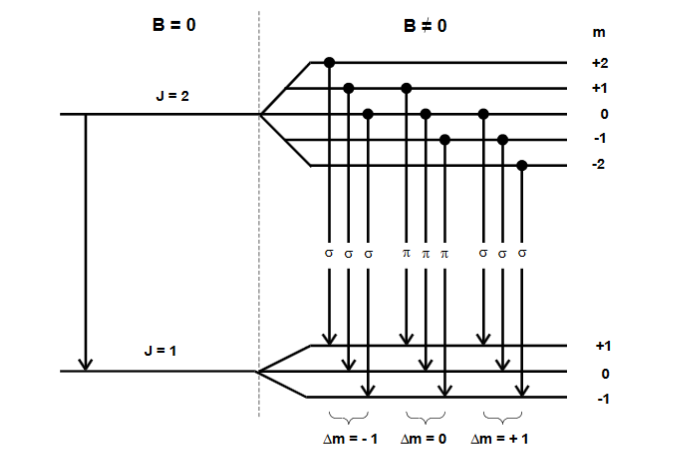
\includegraphics[width=0.8\textwidth]{normal.PNG}
    \caption{Aufspaltung und mögliche Übergänge beim Zeemann-Effekt.\cite{skript}}
    \label{fig:normal}
\end{figure}
Beim normalen Zeemann-Effekt findet grundsätzlich eine Aufspalung in ein Tripplet auf, weil die Energiedifferenzen
innerhalb einer Gruppe mit konstantem $\Delta m$ gleich sind.
Aufgrund der Polarisation sind die Lienien nicht aus jeder Richtung beobachtbar.
Die $\pi$-Linie liegt mit maximaler Intensität senkrecht zur Feldrichtung vor und ist in Feldrichtiung nicht beobachtbar.
Die $\sigma$-Linien erscheinen, senkrecht zur Feldrichtung, ebenfalls linear Polarisiert aber senkrecht zur $\pi$-Linie.
Die Abbildung \ref{fig:aufspaltungsbild} zeigt das Aufspaltungsbild einer Spektrallinie.
\begin{figure}
   \centering
    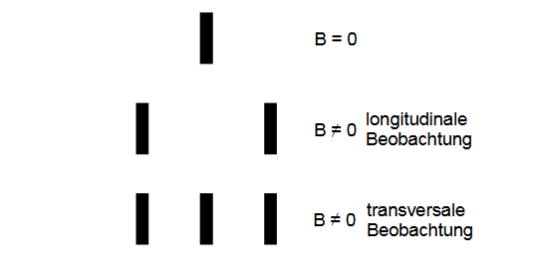
\includegraphics[width=0.7\textwidth]{aufspaltungsbild.PNG}
    \caption{Das Aufspltungsbild einer Spektrallinie.\cite{skript}}
    \label{fig:aufspaltungsbild}
\end{figure}
\subsection{Anomaler Zeemann-Effekt}
Bei dem anomalen Zeemann-Effekt gilt $S \neq 0$ und damit hängen die Energiedifferenzen vom Spin ab.
In diesem Fall ist $g_\mathrm{j}$ nicht automatisch $1$, sondern nimmt verschiedene Werte an.
Die Energieverschiebung ist dann gegeben durch:
\begin{align}
  \Delta E= [m_\mathrm{1}g_\mathrm{J}(L_\mathrm{1},S_\mathrm{1},J_\mathrm{1})]-m_\mathrm{2}g_\mathrm{J}(L_\mathrm{2},S_\mathrm{2},J_\mathrm{2}). \label{eqn:g_ji}
\end{align}
Die Indizes geben die Zordnung zu den Niveaus an.
Die Aufspaltung ist wesentlich Linienreicher und ist in Abbildung \ref{fig:anomal} dargestellt.
\begin{figure}
   \centering
    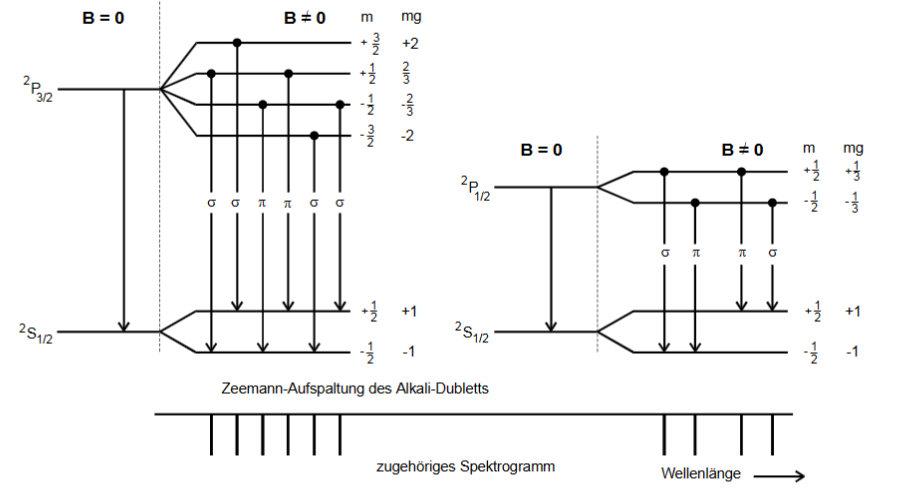
\includegraphics[width=0.8\textwidth]{anomal.PNG}
    \caption{Die Aufspaltung beim anomalen Zeemann-Effekt.\cite{skript}}
    \label{fig:anomal}
\end{figure}
\subsection{Lummer-Gehrcke-Platte}
In diesem Versuch wird zur Sichtbarmachung der Aufspaltung eine Lummer-Gehrke-Platte genutzt.
An dieser Stelle folgt ein kurze Beschreibung der Funktionsweise der Platte.
Eingestrahltes Licht wird innerhalb der Platte mehrfach reflektiert, dabei tritt bei
jeder Reflektion ein Teil des Lichts an der oberen und unteren Grenzfläche aus.
Dies ist in Abbildung $\ref{fig:platte}$ dargestellt.
\begin{figure}
   \centering
    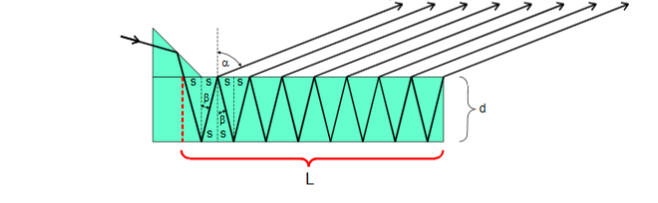
\includegraphics[width=0.9\textwidth]{platte.PNG}
    \caption{Der Strahlengang innerhalb der Lummer-Gehrcke-Platte.\cite{skript}}
    \label{fig:platte}
\end{figure}
Die Strahlen interferieren konstruktiv wenn die Bedingung $2d\cos{\theta}=n\lambda$
erfüllt ist. Hierbei ist $d$ die Dicke der Platte und $\lambda$ die Wellenlänge der Strahlung.
Bei eingeschaltetem Magnetfeld verändert sich die Wellenlänge um $\delta\lambda$ und
die Interferenzstreifen verschieben sich um $\delta s$.
Von Bedeutung sind die beiden Größen Dispersionsgebiet und Auflösungsvermögen.
Das Dispersionsgebiet gibt den Wellenlängendifferenzbereich an, in dem die
Interferenzstreifen sich nicht überlagern:
\begin{align}
  \Delta\lambda_\mathrm{D}=\frac{\lambda^2}{2d}\sqrt{\frac{1}{n^2-1}} \label{eqn:dispersionsgebiet}.
\end{align}
Das Auflösungsvermögen ist durch folgende Beziehung zwischen Brechungsindex $n$,
der Plattenlänge $L$ und der Wellenlänge gegeben:
\begin{align}
  A=\frac{L}{\lambda}(n^2-1)\label{eqn:aufloesung}.
\end{align}

\section{Aufbau und Durchführung}
\label{sec:Durchführung}

\subsection{Justage}
Zu Beginn ist eine Justierung des Interferometers notwendig.
Ziel ist eine Aufspaltung eines Strahls in Zwei Strahlen, die beide in
der horizonthalen Ebene liegen und anschließendes Überlappen der Strahlen
beim Verlassen des Interferometers. Dies wird durch Einstellen der
Spiegel innerhalb und außerhalb des Interferometers erreicht.

Die  Apperatur ist aufgebaut wie in Abbildung \ref{fig:apparat}.
\begin{figure}
    \centering
    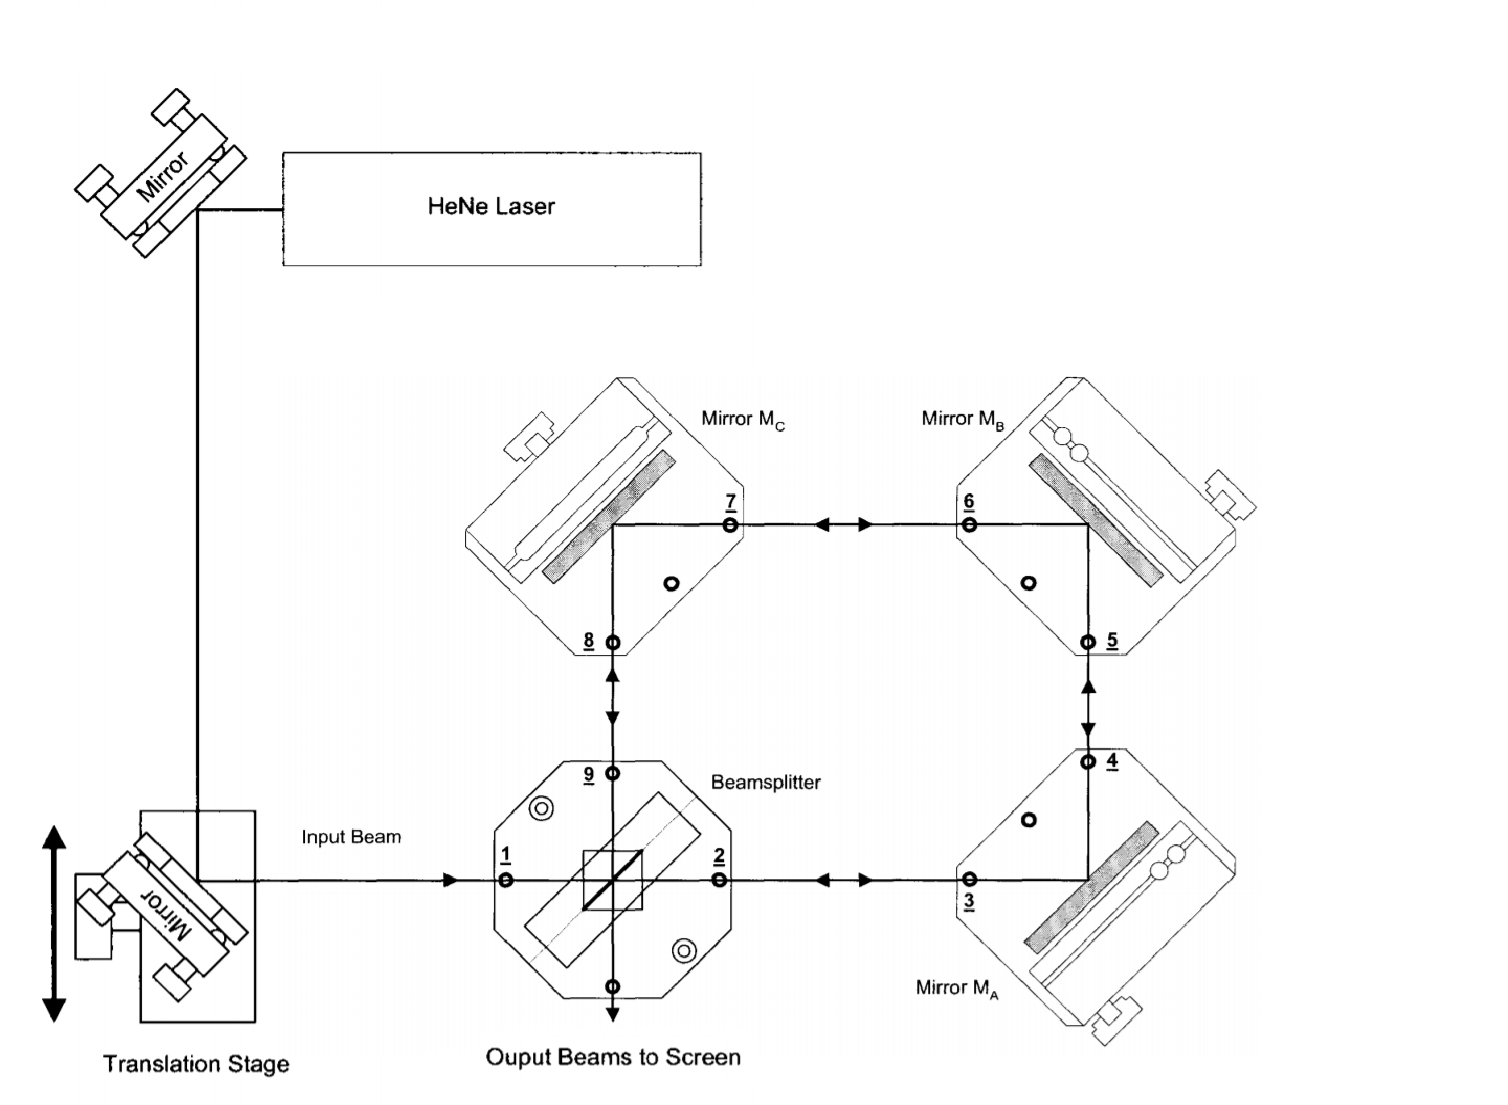
\includegraphics[width=0.7\textwidth]{Apperatur.PNG}
    \caption{Aufbau des Sagnac-Interferometers.\cite{skript}}
    \label{fig:apparat}
\end{figure}
Die Anordnung setzt sich zusammen aus der Quelle, einem HeNe-Laser, zwei
Spiegel zur Ausrichtung des Laserstrahls zum Polarizing-Beam-Splitter-Cube hin.
Zuvor passiert der Laserstrahl einen linearen Polarisationsfilter.
Der PBSC dient zur Aufspaltung des Strahls in Horizntal-und Vertikalkomponente,
dabein passiert die Horizontalkomponente den PBSC und die Vertikalkomponente wird
erfährt einen Richtungsänderung um $90\si{\degree}$. Drei weitere Spiegel lenken
beide Strahle so um, dass diese die gleiche Strecke zurücklegen und wieder auf
den PBSC treffen. Dort werden die Strahlen erneut, nach ihrer polarisation,
umgelenkt und durchgelassen, somit laufen die Strahlen wieder zusammen.
Durch verschieben der Translation Stage können die zwei Strahlen räumlich separiert
werden und somit unterschiedliche Materialien durchqueren.
Bei der ersten Messung werden zwei Glasplättchen, die auf einer Rotationsachse
befestigt sind, unterschiedlicher
Ausrichtung in die beiden Strahlengänge positioniert, zu sehen in der Abbildung
\ref{fig:glasplattchen}.

\begin{figure}
     \centering
     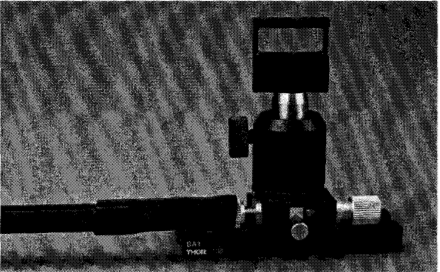
\includegraphics[width=0.7\textwidth]{Glasblattchen.PNG}
     \caption{Rotationsachse mit Glasblättchen.\cite{skript}}
     \label{fig:glasplattchen}
\end{figure}
Zur Messung des Kontrasts wird ein linearer Polarisationsfilter mit $45\si{\degree}$
Ausrichtung verwendet, der hinter dem PBSC positioniert wird.
Dadurch entsteht ein Interferenzbild, dessen Intensität durch eine Photodiode gemessen wird.
Nun wird der Winkel des ersten Polarisationsfilters variiert
und die Glasplättchen so rotiert, dass einmal ein Intensität minima und einmal
ein Intensitäts maxima gemessenwerden kann.

Für die Bestimmung der Brechungsindexe wird der
Winkel des ersten Polarisationsfilters so gewählt, dass ein Kontrast Maximum vorliegt.
des weiteren wird der zweite Polatriationsfilter und die Photodiode entfern.
Statdessen trifft der gebündelte Strahl nun einen Polarisationsseperator realisiert durch einen
weiteren PBSC und einen Spiegel, wie in Abbildung \ref{fig:polsep} zu sehen.
\begin{figure}
     \centering
     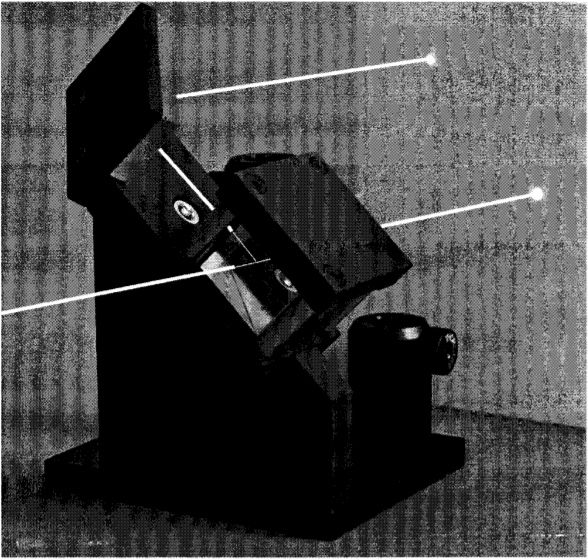
\includegraphics[width=0.7\textwidth]{PSBC.PNG}
     \caption{Aufbau des Polarisationsseperator.\cite{skript}}
     \label{fig:polsep}
\end{figure}

Mittels zweier Photodioden wird der zuvor aufgespaltene Strahl detektiert.
Mit einem Oszilloskop wird die Spannungsdifferenz zwischen den Intensitäten
gemessen. Ein weiteres Gerät zähl die Nulldurchgänge der Spannungsdifferenz.
Bei der Messung für den Brechungsindex von Glas wird
der Winkel der Glasplättchen langsam verändert und die Nulldurchgänge für unterschiedliche
winkel aufgenommen.

Für den Brechnungsindex von Luft werden die Glasplättchen
aus dem Strahlengang enfernt. Es wird eine Gaszelle eingebaut, durch
die nur ein Laserstrahl geht. Die Gaszelle ist verbunden mit einer Pumpe
die ein Vakuum in der Gaszelle erzeugt. Durch ein Ventil wird wieder langsam
Luft in die Zelle gelassen bis wieder der Normaldruck erreicht ist. Während
dieses Vorganges werden wieder Nulldurchgänge von der Spannungsdifferenz aufgenommen.

\section{Auswertung}
\label{sec:Auswertung}
\subsection{Theoretische Werte}
Zu Beginn können mit Hilfe der Formel \eqref{eqn:lande}
die theoretischen Werte der Lande-Faktoren
für die entsprechenden Orbitale ausgerechnet werden.
Die Berechneten Werte sind in der Tabelle \ref{tab:theo1}
zu finden.

\begin{table}
  \centering
  \caption{Theoretische Werte für die Landé-Faktoren der Orbitale.}
  \label{tab:theo1}
  \begin{tabular}{c c c c c c}
    \toprule
& Orbital  & S   &  L & J  & $g_j$ \\
    \midrule
Rot & $^1P_1$ & 0 & 1 & 1 & 1,0\\
&$^1D_2$& 0 & 2 & 2 & 1,0\\
Blau&$^3S_1$& 1 & 0 & 1 & 2,0\\
&$^3P_1$& 1 & 2 & 1 & 1,5\\
    \bottomrule
  \end{tabular}
\end{table}

Deweiteren könnnen die Lané-Faktoren für Übergänge
bei dem anormalen Zeeman-Effekt berechnet werden. Dafür werden nur
Übergänge zwischen Orbitale, die einen Spin $S=!0$, besitzen betrachtet (Blaues Licht).
Die Berechneten Werte sind in der Tabelle \ref{tab:theo2}
zu finden.

\begin{table}
  \centering
  \caption{Theoretische Werte für die Landé-Faktoren $g_{ji}$ für Übergänge bei
  dem der annormale Zeeman-Effekt berücksichtigt werden muss.}
  \label{tab:theo2}
\begin{tabular}{c c c c c c c}
  \toprule
      &            &  \multicolumn{2}{c}{$^3P_1$}  & \multicolumn{2}{c}{$^3P_1$} &    \\
      & $\Delta m$ &   $m_1$&  $m_1g_1$            & $m_2$    & $m_2g_2$         & $g_{ij}$\\
  \midrule
\sigma &  -1   &    1 &  2,0     &  0  & 0,0  &  2,0  \\
       &       &    0 &  0,0     & -1  & 1,5  &  1,5  \\
\pi    &   0   &    1 &  2,0     &  1  & 1,5  &  0,5  \\
       &       &    0 &  0,0     &  0  & 0,0  &  0,0  \\
       &       &   -1 & -2,0     & -1  & -1,5 & -0,5  \\
\sigma &  +1   &    0 &  0,0     &  1  & 1,5  & -1,5  \\
       &       &   -1 & -2,0     &  0  & 0,0  & -2,0  \\
\bottomrule
\end{tabular}
\end{table}

\subsection{Hysterese}
Es wurde eine Hysteresekurve für den verwendeten Elektromagneten aufgenommen.
Die Tabelle \ref{tab:hyst} enthält die Messwerte von des Magnetfeld $B$
in Abhängigkeit von dem  Strom $I$. Diese sind wiederum
in der Abblidung \ref{fig:hyst} aufgetragen.
\begin{table}
  \centering
  \caption{Messwerte für die Hysterese}
  \label{tab:hyst}
\begin{tabular}{c c c c}
  \toprule
 Strom $I/\si{\ampere}$ & Magnetfeld $B/\si{\milli\tesla}$  & $I/\si{\ampere}$ & $B/\si{\milli\tesla}$ \\
  \midrule
%messwerte
  \bottomrule
\end{tabular}
\end{table}


% \begin{figure}
%   \centering
%   \includegrafics{}
%   \caption
%   \label{fig:hyst}
% \end{figure}

Um Später die Benötigten B-Felder Zu bestimmen wird eine Ausgleichsrechnung
an den Messwerten bei steigendem Strom durch geführt.
Als Ansatz wird die Funktion
\begin{align}
B(I)=A \cdot \arctan(\frac{I-I_0}/C) \label{eqn:hyst}
\end{align}
verwendet.
Es ergeben sich für die Parameter die folgenden Werte:
\begin{align}
  A=\SI{1.39(7)e3}{\milli\tesla}   & I_0=\SI{0.21(13)}{\ampere}  &  C=\SI{21.6(16)}{ampere}
\end{align}

\newpage
\section{Diskussion}
\label{sec:Diskussion}
Die Messung der Brechungsindices von Glas
und Luft liefert folgende Ergebnisse:
\begin{align*}
  n_\mathrm{Glas}&=1,18\pm0,04\\
  n_\mathrm{Luft}&=1,000264\pm 3\dot10^{-6}.
\end{align*}
Werden diese mit den Literaturwerten
\begin{align*}
n_{\mathrm{lit}_\mathrm{Glas}}&=1,45  \ \ \ \text{\cite{literatur}}\\
n_{\mathrm{lit}_\mathrm{Luft}}&=1,000292     \ \ \ \text{\cite{literatur}}
\intertext{verglichen, ergeben sich die entsprechenden Abweichungen:}
a_\mathrm{Glas}&\approx0,18\\
a_\mathrm{Luft}&\approx2,8\cdot 10^{-5}.
\end{align*}
Die etwas höhere Abweichung bei dem Brechungsindex von Glas
im Gegensatzt zu Luft, lässt sich möglicherweise durch die
Nährung in der Formel
\eqref{eqn:glas} begründen. Bei der Formel wird angenommen, dass nur ein Laserstrahl
eine Glasplatte passiert. Jedoch passieren in dem Experiment beide Laserstrahlen
zwei unterschiedlich ausgerichtete Glasplatten, wobei ein Winkel von einer Glasplatte gegen
$0 \si{\degree}$ geht. Folglich ist die zweite Glasplatte nicht
vernachlässigbar und muss in der Formel berücksichtigt werden. Diese Korrektur könne
für besser Ergebnisse bei dem Brechungsindex für Glas führen. Die Messung des Brechungsindex
von Luft liefert recht genau Ergebnisse, was für die Präzision des Sagnac-Interferometer spricht.

\section{Anhang}
\label{sec:anhang}
\subsection{Fehlerrechnung}
Die Mittelwerte bestimmen sich in der Auswertung nach:
\begin{align}
  \bar{x}=\frac{1}{n} \sum_{i=1}^n x_i\,.
\end{align}
Für die Standardabweichung ergibt sich:
\begin{align}
 s_i=\sqrt{\frac{1}{n-1}\sum_{j=1}^n (v_j-\bar{v_i})^2}
\end{align}
mit $v_j$ mit $j=1,..,n$ als Wert mit zufällig behafteten Fehlern.\\
Diese werden mit Hilfe von
Numpy 1.9.2, einer Erweiterung von Python 3.2.0, berechnet.
Die Fehlerfortpflanzung wird mit der Gauß´schen Fehlerfortpflanzung berechnet
 \eqref{eqn:gaus}.
\begin{equation}
\Delta f=\sqrt{\sum_{j=1}^n \left(\frac{\partial f}{\partial x_j}\Delta x_j \right)^{2} }\label{eqn:gaus}.
\end{equation}
Diese wird von der Erweiterung Uncertainties 2.4.6.1 von Python 3.2.0 übernommen.
Desweitern wird in der Auswertung Lineare Regression benutzt.
um die Konstanten A und B aus einen Gleichung der Form
\begin{align}
  y(x)=&A+B\cdot x\label{eqn:lin}
\intertext{zu berechnen. B errechnet sich hierbei aus der Formel}
B&=\frac{\overline{xy}-\overline{x}\cdot \overline{y}}{\overline{x^2}-\overline{x}^2}.
\intertext{und A durch die Geleichung }\\
A&=\overline{y}-B\cdot \overline{x}\,.\\
\intertext{Die Ungenauigkeit von A und B ergibt sich aus der
mittleren Streuung:}\\
s_{\mathrm{y}}&=\sqrt{\frac{1}{N-2}\cdot \sum_{i=1}^{N}\left(y_i-A-B\cdot x_i\right)^2}\,.\\
\intertext{Für die Ungenauigkeit von B gilt:}\\
s_{\mathrm{B}}&=s_{\mathrm{y}} \cdot \sqrt{\frac{1}{N \cdot \left(\overline{x^2}-\left(\overline{x}\right)^2\right)}}\,.\\
\intertext{Für die Ungenauigkeit von A gilt:}\\
s_{\mathrm{A}}&=s_{\mathrm{B}} \cdot\sqrt{\overline{x^2}}\,.
\end{align}
Für die Lineare Regression wird die Erweiterung Scipy 0.15.1 für Python 3.2.0
benutzt.
Abweichungen von den Theoriewerten werden mit der Formel
\begin{align}
  a=\frac{|a_\mathrm{gemessen}-a_\mathrm{theorie}|}{a_\mathrm{theorie}} \label{eqn:abweich}
\end{align}
berechnet.

\printbibliography
\subsection{Messwerte}
\label{sec:mess}
\begin{longtable}{cc}
  \caption{Messwerte für die Intensitätsverteilung bei $I=\SI{0.4}{\ampere}$.}\\
  \hline
  \toprule
  Spindelumdrehungen $/Skt$ & Intensität $/\si{\milli\volt}$ \\
  \midrule
\endfirsthead
\toprule
Spindelumdrehungen $/Skt$ & Intensität $/\si{\milli\volt}$ \\
\midrule
\endhead
\bottomrule
\endfoot
\bottomrule
\bottomrule
\endlastfoot
3,8  & 133\\
3,9  & 134\\
4,0  & 135\\
4,1  & 137\\
4,2  & 138\\
4,3  & 141\\
4,4  & 144\\
4,5  & 150\\
4,6  & 154\\
4,7  & 158\\
4,8  & 164\\
4,85 & 167\\
4,9  & 169\\
4,95 & 172\\
5,0  & 174\\
5,05 & 178\\
5,1  & 182\\
5,15 & 190\\
5,2  & 195\\
5,25 & 199\\
5,3  & 205\\
5,35 & 210\\
5,4  & 218\\
5,45 & 227\\
5,5  & 232\\
5,55 & 242\\
5,6  & 250\\
5,65 & 268\\
5,7  & 279\\
5,75 & 292\\
5,8  & 303\\
5,85 & 317\\
5,9  & 332\\
5,95 & 348\\
6,0  & 360\\
6,05 & 372\\
6,1  & 387\\
6,15 & 392\\
6,2  & 395\\
6,25 & 395\\
6,3  & 387\\
6,35 & 378\\
6,4  & 360\\
6,45 & 343\\
6,5  & 320\\
6,55 & 298\\
6,6  & 280\\
6,65 & 267\\
6,7  & 255\\
6,75 & 254\\
6,8  & 259\\
6,85 & 269\\
6,9  & 282\\
6,95 & 294\\
7,0  & 310\\
7,05 & 322\\
7,1  & 337\\
7,15 & 349\\
7,2  & 359\\
7,25 & 365\\
7,3  & 370\\
7,35 & 372\\
7,4  & 370\\
7,45 & 364\\
7,5  & 355\\
7,55 & 343\\
7,6  & 330\\
7,65 & 313\\
7,7  & 290\\
7,75 & 288\\
7,8  & 277\\
7,85 & 265\\
7,9  & 256\\
7,95 & 246\\
8,0  & 236\\
8,05 & 232\\
8,1  & 225\\
8,15 & 219\\
8,2  & 215\\
8,25 & 210\\
8,3  & 204\\
8,35 & 199\\
8,4  & 194\\
8,45 & 191\\
8,5  & 186\\
8,55 & 180\\
8,6  & 177\\
8,65 & 174\\
8,7  & 170\\
8,75 & 166\\
8,8  & 162\\
8,9  & 158\\
9,0  & 153\\
9,1  & 150\\
9,2  & 148\\
9,3  & 143\\
9,4  & 140\\
9,5  & 136\\
9,6  & 136\\
9,7  & 133\\
9,8  & 130\\
9,9  & 129\\
10   & 128\\
%\bottomrule
\end{longtable}

\begin{longtable}{cc}
  \caption{Messwerte für die Intensitätsverteilung bei $I=\SI{0.5}{\ampere}$.}\\
  \hline
  \toprule
  Spindelumdrehungen $/Skt$ & Intensität $/\si{\milli\volt}$ \\
  \midrule
\endfirsthead
\toprule
Spindelumdrehungen $/Skt$ & Intensität $/\si{\milli\volt}$ \\
\midrule
\endhead
\bottomrule
\endfoot
\bottomrule
\bottomrule
\endlastfoot
3,8 & 132\\
3,9 & 135\\
4,0 & 138\\
4,1 & 142\\
4,2 & 144\\
4,3 & 147\\
4,4 & 150\\
4,5 & 155\\
4,6 & 162\\
4,7 & 171\\
4,8 & 176\\
4,9 & 182\\
4,95& 189\\
5,0 & 190\\
5,05& 196\\
5,1 & 198\\
5,15& 203\\
5,2 & 208\\
5,25& 216\\
5,3 & 222\\
5,35& 224\\
5,4 & 229\\
5,45& 239\\
5,5 & 249\\
5,55& 258\\
5,6 & 272\\
5,65& 283\\
5,7 & 294\\
5,75& 309\\
5,8 & 317\\
5,85& 330\\
5,9 & 339\\
5,95& 349\\
6,0 & 361\\
6,05& 367\\
6,1 & 370\\
6,15& 370\\
6,2 & 367\\
6,25& 358\\
6,3 & 347\\
6,35& 334\\
6,4 & 308\\
6,45& 288\\
6,5 & 268\\
6,55& 246\\
6,6 & 229\\
6,65& 217\\
6,7 & 212\\
6,75& 216\\
6,8 & 224\\
6,85& 236\\
6,9 & 249\\
6,95& 264\\
7,0 & 277\\
7,05& 286\\
7,1 & 301\\
7,15& 313\\
7,2 & 324\\
7,25& 335\\
7,3 & 341\\
7,35& 347\\
7,4 & 352\\
7,45& 346\\
7,5 & 344\\
7,55& 336\\
7,6 & 328\\
7,65& 320\\
7,7 & 307\\
7,75& 292\\
7,8 & 286\\
7,85& 276\\
7,9 & 269\\
7,95& 261\\
8,0 & 254\\
8,05& 246\\
8,1 & 236\\
8,15& 231\\
8,2 & 221\\
8,25& 216\\
8,3 & 209\\
8,35& 208\\
8,4 & 201\\
8,45& 200\\
8,5 & 195\\
8,55& 191\\
8,6 & 186\\
8,65& 183\\
8,7 & 179\\
8,8 & 174\\
8,9 & 169\\
9,0 & 166\\
9,1 & 159\\
9,2 & 153\\
9,3 & 150\\
9,4 & 146\\
9,5 & 142\\
9,6 & 140\\
9,7 & 137\\
9,8 & 135\\
\end{longtable}

\begin{longtable}{cc}
  \caption{Messwerte für die Intensitätsverteilung bei $I=\SI{0.6}{\ampere}$.}\\
  \hline
  \toprule
  Spindelumdrehungen $/Skt$ & Intensität $/\si{\milli\volt}$ \\
  \midrule
\endfirsthead
\toprule
Spindelumdrehungen $/Skt$ & Intensität $/\si{\milli\volt}$ \\
\midrule
\endhead
\bottomrule
\endfoot
\bottomrule
\bottomrule
\endlastfoot
3,3  & 133\\
3,4  & 134\\
3,5  & 133\\
3,6  & 137\\
3,7  & 140\\
3,8  & 142\\
3,9  & 147\\
4,0  & 150\\
4,1  & 153\\
4,2  & 158\\
4,3  & 162\\
4,4  & 165\\
4,5  & 170\\
4,6  & 175\\
4,7  & 180\\
4,8  & 187\\
4,9  & 192\\
4,95 & 196\\
5,0  & 201\\
5,05 & 205\\
5,1  & 209\\
5,15 & 212\\
5,2  & 218\\
5,25 & 224\\
5,3  & 229\\
5,35 & 239\\
5,4  & 244\\
5,45 & 253\\
5,5  & 264\\
5,55 & 274\\
5,6  & 283\\
5,65 & 291\\
5,7  & 301\\
5,75 & 313\\
5,8  & 322\\
5,85 & 329\\
5,9  & 337\\
5,95 & 339\\
6,0  & 343\\
6,05 & 344\\
6,1  & 339\\
6,15 & 331\\
6,2  & 325\\
6,25 & 314\\
6,3  & 299\\
6,35 & 277\\
6,4  & 258\\
6,45 & 242\\
6,5  & 221\\
6,55 & 205\\
6,6  & 194\\
6,65 & 189\\
6,7  & 182\\
6,75 & 188\\
6,8  & 194\\
6,85 & 204\\
6,9  & 216\\
6,95 & 229\\
7,0  & 240\\
7,05 & 249\\
7,1  & 264\\
7,15 & 272\\
7,2  & 287\\
7,25 & 296\\
7,3  & 307\\
7,35 & 314\\
7,4  & 319\\
7,45 & 323\\
7,5  & 325\\
7,55 & 320\\
7,6  & 317\\
7,65 & 312\\
7,7  & 303\\
7,75 & 294\\
7,8  & 287\\
7,85 & 280\\
7,9  & 271\\
7,95 & 265\\
8,0  & 260\\
8,05 & 250\\
8,1  & 244\\
8,15 & 238\\
8,2  & 234\\
8,25 & 229\\
8,3  & 230\\
8,35 & 220\\
8,4  & 216\\
8,45 & 210\\
8,5  & 203\\
8,55 & 199\\
8,6  & 194\\
8,65 & 187\\
8,7  & 188\\
8,8  & 180\\
8,9  & 173\\
9,0  & 170\\
9,1  & 165\\
9,2  & 162\\
9,3  & 157\\
9,4  & 155\\
9,5  & 150\\
9,6  & 146\\
9,7  & 142\\
9,8  & 139\\
9,9  & 139\\
10,0 & 138\\
\end{longtable}

\begin{longtable}{cc}
  \caption{Messwerte für die Intensitätsverteilung bei $I=\SI{0.735}{\ampere}$.}\\
  \hline
  \toprule
  Spindelumdrehungen $/Skt$ & Intensität $/\si{\milli\volt}$ \\
  \midrule
\endfirsthead
\toprule
Spindelumdrehungen $/Skt$ & Intensität $/\si{\milli\volt}$ \\
\midrule
\endhead
\bottomrule
\endfoot
\bottomrule
\bottomrule
\endlastfoot
3,3  & 130\\
3,4  & 131\\
3,5  & 133\\
3,6  & 137\\
3,7  & 140\\
3,8  & 144\\
3,9  & 146\\
4,0  & 149\\
4,1  & 151\\
4,2  & 157\\
4,3  & 161\\
4,4  & 167\\
4,5  & 174\\
4,6  & 180\\
4,7  & 185\\
4,8  & 193\\
4,85 & 196\\
4,9  & 200\\
4,95 & 203\\
5,0  & 209\\
5,05 & 213\\
5,1  & 216\\
5,15 & 222\\
5,25 & 229\\
5,3  & 236\\
5,35 & 244\\
5,4  & 252\\
5,45 & 260\\
5,5  & 269\\
5,55 & 278\\
5,6  & 288\\
5,65 & 295\\
5,7  & 302\\
5,75 & 305\\
5,8  & 310\\
5,85 & 312\\
5,9  & 315\\
5,95 & 316\\
6,0  & 310\\
6,05 & 305\\
6,1  & 299\\
6,15 & 290\\
6,2  & 278\\
6,25 & 266\\
6,3  & 250\\
6,35 & 236\\
6,4  & 218\\
6,45 & 201\\
6,5  & 187\\
6,55 & 174\\
6,6  & 164\\
5,2 228
6,65 & 157\\
6,7  & 160\\
6,75 & 163\\
6,8  & 170\\
6,85 & 180\\
6,9  & 191\\
6,95 & 199\\
7,0  & 209\\
7,05 & 218\\
7,1  & 227\\
7,15 & 238\\
7,2  & 253\\
7,25 & 264\\
7,3  & 270\\
7,35 & 280\\
7,4  & 290\\
7,45 & 299\\
7,5  & 302\\
7,55 & 304\\
7,6  & 302\\
7,65 & 294\\
7,7  & 289\\
7,75 & 285\\
7,8  & 280\\
7,85 & 273\\
7,9  & 267\\
7,95 & 264\\
8,0  & 258\\
8,05 &256\\
8,1  &255\\
8,15 &250\\
8,2  &244\\
8,25 &240\\
8,3  &243\\
8,35 &229\\
8,4  &224\\
8,45 &219\\
8,5  &214\\
8,55 &208\\
8,6  &202\\
8,65 &199\\
8,7  &194\\
8,8  &190\\
8,9  &184\\
9,0  &178\\
9,1  &171\\
9,2  &166\\
9,3  &162\\
9,4  &153\\
9,5  &151\\
9,6  &146\\
9,7  &144\\
9,8  &141\\
9,9  &140\\
10,0 &137\\
10,1 &136\\
10,2 &137\\
\end{longtable}

\begin{longtable}{cc}
  \caption{Messwerte für die Intensitätsverteilung bei $I=\SI{0.8}{\ampere}$.}\\
  \hline
  \toprule
  Spindelumdrehungen $/Skt$ & Intensität $/\si{\milli\volt}$ \\
  \midrule
\endfirsthead
\toprule
Spindelumdrehungen $/Skt$ & Intensität $/\si{\milli\volt}$ \\
\midrule
\endhead
\bottomrule
\endfoot
\bottomrule
\bottomrule
\endlastfoot
3,3 &131\\
3,4 &134\\
3,5 &137\\
3,6 &140\\
3,7 &142\\
3,8 &146\\
3,9 &148\\
4,0 & 152\\
4,1 & 156\\
4,2 & 161\\
4,3 & 163\\
4,4 & 169\\
4,5 & 175\\
4,6  &183\\
4,7  &193\\
4,8  &199\\
4,85 &202\\
4,9  &206\\
4,95 &210\\
5,0  &213\\
5,05 &219\\
5,1  &226\\
5,15 &229\\
5,2  &233\\
5,25 &242\\
5,3  &244\\
5,35 &248\\
5,4  &257\\
5,45 &264\\
5,5  &271\\
5,55 &284\\
5,6  &287\\
5,65 &296\\
5,7  &302\\
5,75 &308\\
5,8  &306\\
5,85 &308\\
5,9  &307\\
5,95 &305\\
6,0  &300\\
6,05 &296\\
6,1  &286\\
6,15 &277\\
6,2  &267\\
6,25 &252\\
6,3  &219\\
6,35 &207\\
6,4  &193\\
6,45 &178\\
6,5  &167\\
6,55 &158\\
6,6  &154\\
6,65 &154\\
6,7  &156\\
6,75 &161\\
6,8  &171\\
6,85 &176\\
6,9  &187\\
6,95 &195\\
7,0  & 203\\
7,05 &214\\
7,1  &223 \\
7,15 &234\\
7,2  &245\\
7,25 &256\\
7,3  &265\\
7,35 &272\\
7,4  &279\\
7,45 &285\\
7,5  &289\\
7,55 &289\\
7,6  &292\\
7,65 &288\\
7,7  &281\\
7,75 &280\\
7,8  &276\\
7,85 &272\\
7,9  &267\\
7,95 &263\\
8,0  &261\\
8,05 &253\\
8,1  &250\\
8,15 &245\\
8,2  &239\\
8,25 &231\\
8,3  &227\\
8,35 &222\\
8,4  &215\\
8,45 &210\\
8,5  &206\\
8,55 &202\\
8,6  &198\\
8,65 & 193\\
8,7  & 186\\
8,8  & 178\\
8,9  & 175\\
9,0  & 171\\
9,1  & 166\\
9,2  & 162\\
9,3  & 157\\
9,4  & 154\\
9,5  & 149\\
9,6  & 146\\
9,7  & 140\\
9,8  & 140\\
9,9  & 137\\
10,0 & 135\\
10,1 & 134\\
\end{longtable}

\begin{longtable}{cc}
  \caption{Messwerte für die Intensitätsverteilung bei $I=\SI{0.91}{\ampere}$.}\\
  \hline
  \toprule
  Spindelumdrehungen $/Skt$ & Intensität $/\si{\milli\volt}$ \\
  \midrule
\endfirsthead
\toprule
Spindelumdrehungen $/Skt$ & Intensität $/\si{\milli\volt}$ \\
\midrule
\endhead
\bottomrule
\endfoot
\bottomrule
\bottomrule
\endlastfoot
3,3 & 136\\
3,4 & 137\\
3,5 & 138\\
3,6 & 142\\
3,7 & 146\\
3,8 & 151\\
3,9 & 153\\
4,0  & 158\\
4,1  & 163\\
4,2  & 166\\
4,3  & 171\\
4,4  & 177\\
4,5  & 184\\
4,6  & 191\\
4,7  & 195\\
4,75 & 199\\
4,8  & 205\\
4,85 & 209\\
4,9  & 210\\
4,95 & 214\\
5,0  & 218\\
5,05 & 222\\
5,1  & 226\\
5,15 & 232\\
5,2  & 238\\
5,25 & 241\\
5,3  & 247\\
5,35 & 252\\
5,4  & 258\\
5,45 & 263\\
5,5  & 269\\
5,55 & 274\\
5,6  & 278\\
5,65 & 284\\
5,7  & 289\\
5,75 & 289\\
5,8  & 286\\
5,85 & 284\\
5,9  & 282\\
5,95 & 276\\
6,0  & 272\\
6,05 & 264\\
6,1  & 256\\
6,15 & 246\\
6,2  & 234\\
6,25 & 218\\
6,3  & 206\\
6,35 & 195\\
6,4  & 184\\
6,45 & 170\\
6,5  & 162\\
6,55 & 153\\
6,6  & 149\\
6,65 & 144\\
6,7  & 144\\
6,75 & 146\\
6,8  & 151\\
6,85 & 156\\
6,9  & 162\\
6,95 & 167\\
7,0  & 178\\
7,05 & 184\\
7,1  & 193\\
7,15 & 202\\
7,2  & 212\\
7,25 & 218\\
7,3  & 232\\
7,35 & 240\\
7,4  & 246\\
7,45 & 255\\
7,5  & 263\\
7,55 & 268\\
7,6  & 273\\
7,65 & 274\\
7,7  & 274\\
7,75 & 272\\
7,8  & 271\\
7,85 & 269\\
7,9  & 266\\
7,95 & 264\\
8,0  & 255\\
8,05 & 250\\
8,1  & 249\\
8,15 & 246\\
8,2  & 244\\
8,25 & 238\\
8,3  & 232\\
8,35 & 228\\
8,4  & 226\\
8,45 & 221\\
8,5  & 216\\
8,55 & 212\\
8,6  & 207\\
8,65 & 203\\
8,7  & 200\\
8,75 & 196\\
8,8  & 192\\
8,9  & 187\\
9,0  & 183\\
9,1  & 178\\
9,2  & 172\\
9,3  & 169\\
9,4  & 162\\
9,5  & 157\\
9,6  & 156\\
9,7  & 152\\
9,8  & 150\\
9,9  & 146\\
10,0 & 144\\
10,1 & 143\\
10,2 & 140\\
10,3 & 140\\
10,4 & 137\\
10,5 & 133\\
\end{longtable}


\end{document}
